% ---------------------------------------------------------------------------
% RateCert-HEP -- manuscript for Computer Physics Communications (CPC).
% Converted from the SciPost Physics Codebases submission dated 2026-09-12.
%
% The science, statistics, benchmark numbers and measured timings are unchanged
% from the reviewed SciPost version.  Changes are confined to: CPC class and
% front matter, the mandatory Program Summary, keyword and declaration blocks,
% physics-scope framing, and positioning against prior CPC limit-setting tools.
%
% BUILD:  pdflatex -> bibtex -> pdflatex -> pdflatex
% ---------------------------------------------------------------------------
\documentclass[preprint,12pt]{elsarticle}

\usepackage{amsmath,amssymb}
\usepackage{graphicx}
\usepackage{booktabs}
\usepackage{siunitx}
\usepackage{url}
\usepackage{textcomp}
\graphicspath{{figures/}{../reports/figures/}}

%% Numbered list environment for the Program Summary's own reference list,
%% taken from the official CPC CPiP template (cpc-cpip-template.tex).
\newcounter{bla}
\newenvironment{refnummer}{%
\list{[\arabic{bla}]}%
{\usecounter{bla}%
 \setlength{\itemindent}{0pt}%
 \setlength{\topsep}{0pt}%
 \setlength{\itemsep}{0pt}%
 \setlength{\labelsep}{2pt}%
 \setlength{\listparindent}{0pt}%
 \settowidth{\labelwidth}{[9]}%
 \setlength{\leftmargin}{\labelwidth}%
 \addtolength{\leftmargin}{\labelsep}%
 \setlength{\rightmargin}{0pt}}}
 {\endlist}

\journal{Computer Physics Communications}

\begin{document}

\begin{frontmatter}

\title{RateCert-HEP: a program for finite-sample certification of
fixed-point trigger rates}

\author[hebut]{Jiahui Wu}
\author[hongyang]{Chong Liu}
\author[hongyang]{Tuo Li}
\author[hongyang]{Lei Lv}
\author[hongyang]{Pengjie Guo}
\author[hongyang]{Guoquan Zhang}
\author[hebut]{Jianfeng Sun\corref{cor1}}
\cortext[cor1]{Corresponding author.}
\ead{sunjianfeng10@hebut.edu.cn}

\address[hebut]{School of Materials Science and Engineering, Hebei University of
Technology, Tianjin 300401, China}
\address[hongyang]{Hongyang Display (Xianyang) Technology Co., Ltd.,
Xianyang 712000, Shaanxi, China}

\begin{abstract}
Trigger scores used in high-energy-physics pipelines are often calibrated with
finite samples and then represented by fixed-point firmware registers.  A small
empirical tail, however, does not by itself certify a rate budget, and a rate
register least-significant bit is not a bound on the change induced by score
quantization.  We present RateCert-HEP, a model-agnostic program that keeps
these quantities separate.  It selects an integer threshold on a calibration
block, applies an exact one-sided finite-sample bound on an independent
deployment block, and checks a declared rate-register resolution and counter
full scale.  When only public fixed-size event samples are available, the same
application programming interface reports a binomial background-acceptance
probability and refuses to invent an absolute Hz value.  On the LHC Olympics
2020 R\&D feature release, a family-wise 1\% sweep over 27 score-width,
deployment-prefix, and acceptance-target cells certified 19 cells.  A separate
Poisson benchmark certified 11 of 36 explicit-exposure rate cells.  An
independent 20{,}000-repeat finite-sample coverage stress test observed
coverage of at least 0.99945 at the per-cell confidence used in the public-data
sweep.  The package records machine-readable provenance, refusal reasons, and
quantization diagnostics.  Applied to the same 27 deployment cells, reporting
the empirical tail as an upper bound certifies all 27 while attaining only
about 0.51--0.56 coverage against a nominal 0.9996, whereas the exact bound
holds its nominal coverage; a one-sided normal bound under-covers at small
counts yet certifies more cells than the exact construction, which is exactly
backwards.  RateCert-HEP provides a reproducible statistical contract
conditional on the declared sampling model; it is not a detector-hardware
timing or live-rate measurement.

% ---------------------------------------------------------------------------
% PROGRAM SUMMARY -- mandatory for CPC Computer Programs in Physics (CPiP)
% articles.  Placed immediately following the abstract, inside the abstract
% environment, exactly as required by the official CPC CPiP LaTeX template.
% Fields follow the current official template; the legacy fields used by older
% CPC papers (e.g. TRolke 2.0, 2010) are no longer part of it.
% ---------------------------------------------------------------------------
\vspace{6pt}
\noindent\rule{\textwidth}{0.4pt}
\vspace{4pt}

\noindent\textbf{PROGRAM SUMMARY}

\begin{small}
\noindent
{\em Program Title:} RateCert-HEP \\
{\em CPC Library link to program files:} (to be added by Technical Editor) \\
{\em Developer's repository link:} \url{https://github.com/pixele8/ratecert-hep} \\
{\em Licensing provisions (please choose one):} MIT \\
{\em Programming language:} Python 3 \\
{\em Supplementary material:} None.  The manuscript, test suite, benchmark
scripts and pre-generated figure files are contained in the repository above. \\
{\em Nature of problem (approx.\ 50--250 words):}
A real-time trigger must be configured against a rate budget, but the number
that appears in the firmware is not the number that was statistically
certified.  Three distinct quantities are routinely conflated: (i) the
threshold is chosen from a finite calibration sample, so the empirical tail is
not a probability; (ii) the deployment rate is observed over a finite exposure
or a fixed-size event sample, so the observed count is not the true rate; and
(iii) the rate is stored in a counter or register of finite resolution, so a
register least-significant bit (LSB) is a representation step and not a bound on
the change induced in the rate by score quantization.  Treating any one of
these as exact can make a trigger menu appear to satisfy its budget while
leaving no statistical or numerical margin.  Existing limit-setting programs
return a confidence interval for a count, but they are not attached to the
provenance of that count, to the identity of the sample that selected the
threshold, or to the finite resolution of the register that will store the
result. \\
{\em Solution method (approx.\ 50--250 words):}
Exact frequentist tail inversion.  The three quantities are kept as
independently declared objects joined by a single pass predicate.  Threshold
selection consumes only the calibration block; the selected integer code is
frozen and the deployment block is evaluated afterwards.  With a known exposure
$T$ and observed count $N$ the program returns the exact one-sided Poisson
upper limit $U_\alpha(N,T)=\chi^2_{1-\alpha,2(N+1)}/2T$; with only a fixed-size
sample of $n$ events of which $K$ pass, it returns the exact one-sided
Clopper--Pearson binomial limit
$U_\alpha(K,n)=\mathrm{Beta}^{-1}(1-\alpha;K+1,n-K)$ [1].  Both are evaluated
through survival functions (\texttt{chi2.isf}, \texttt{beta.isf}) rather than by
forming an inverse cumulative distribution at $1-\alpha$, which preserves
precision after a family-wise alpha split.  The rate-register declaration
contributes a deterministic rounding margin ($\Delta_r/2$ for nearest-even,
$\Delta_r$ for floor or truncation) and a counter full-scale range predicate,
both kept strictly separate from the statistical bound.  Score quantization is
audited by a distribution-specific diagnostic that is never promoted to a
universal error bound.  The qualifying configuration satisfies
$U_\alpha+\delta_r\le R_{\mathrm{budget}}$; a configuration that fails is
retained as a valid structured \texttt{NOT\_CERTIFIED} record with explicit
reasons rather than discarded. \\
{\em Additional comments including restrictions and unusual features
(approx.\ 50--250 words):}
The program is model-agnostic: it accepts a caller-supplied score stream and
does not train, replace, or benchmark a classifier.  It does not choose a
physics observable, estimate a detector cross section, infer live time from the
row count of a Monte Carlo file, or synthesize an FPGA design.  When only a
public fixed-size sample is available it deliberately refuses to emit an
absolute Hz field unless an external input flux and rate budget are supplied
together.  The finite-sample guarantee is conditional on the declared sampling
model; the program ships an executable demonstration of this boundary in which
bursty and mixed-rate windows with the same nominal mean are correctly refused.
The program is a reference implementation: on the reference platform it
requires 2.4\,ms to quantize and 2.8\,ms to certify a $10^5$-event acceptance
certificate, and 7.2\,ms for an explicit-exposure rate certificate including
the attainable threshold curve.  These are CPython throughput measurements and
do not represent detector or firmware latency.  Core dependencies are NumPy and
SciPy; pandas/PyTables are required only for the HDF5 public-data adapter and
Matplotlib only for the figure scripts.

\vspace{2pt}
\begin{refnummer}
\item C.~J. Clopper and E.~S. Pearson, \textit{The use of confidence or
fiducial limits illustrated in the case of the binomial}, Biometrika
\textbf{26} (1934) 404--413.
\item J.~Lundberg, J.~Conrad, W.~Rolke and A.~Lopez, \textit{Limits, discovery
and cut optimization for a Poisson process with uncertainty in background and
signal efficiency: TRolke 2.0}, Comput.\ Phys.\ Commun.\ \textbf{181} (2010)
683--686.
\item J.~Conrad, \textit{A program for confidence interval calculations for a
Poisson process with background including systematic uncertainties: POLE 1.0},
Comput.\ Phys.\ Commun.\ \textbf{158} (2004) 117--123.
\end{refnummer}
\end{small}

\vspace{4pt}
\end{abstract}

\begin{keyword}
Trigger rate \sep Fixed-point arithmetic \sep Finite-sample confidence bound \sep
Poisson upper limit
\end{keyword}

\end{frontmatter}

% ---------------------------------------------------------------------------
\section{Introduction}
\label{sec:intro}

Real-time trigger systems must make a discrete decision under a rate budget.
The decision is usually produced by a score whose numerical representation is
fixed before deployment.  Three sources of uncertainty are then coupled in
practice: the threshold is selected from a finite calibration sample, the
deployment rate is observed over a finite exposure, and the rate is stored in a
counter or register with finite resolution.  Treating an empirical tail as an
exact probability, or treating a rate-register LSB as a score-quantization
bound, can make a configuration appear safe while leaving no statistical or
numeric margin.

The practical setting is the one familiar from collider trigger menus.  A
level-1 or high-level trigger stage has a fixed output rate allocation, and each
trigger signature consumes part of it.  Once a menu entry is accepted, its
threshold is committed to firmware, where the score is carried in a fixed-point
format of a few bits to meet latency and resource constraints; the same
constraint has motivated a continuing line of FPGA and high-level-synthesis work
reported in this journal, from integer-arithmetic implementations to recent
HLS-based HEP algorithm acceleration~\cite{Wojenski2024HLS} and deep-learning
triggers~\cite{Tyson2023CLAS12}.  The rate that finally appears in the counter
is therefore the composition of a statistic evaluated on a finite sample, a
quantization of the score, and a rounding of the recorded rate.

Prior work in this journal has addressed the statistical half of this problem
well, and over a long period: POLE 1.0~\cite{Conrad2004POLE} and
TRolke 2.0~\cite{Lundberg2010TRolke} provide exact confidence intervals and
upper limits for a Poisson process, including systematic uncertainties;
Aguilar-Saavedra~\cite{AguilarSaavedra2000} and Barlow~\cite{Barlow2002}
supply dedicated interval calculators; and the Bayesian analysis
toolkit~\cite{BAT2009} generalises the treatment to a full posterior.  These
programs, however, return a number for a statistic.  They do not know whether
the threshold that produced the observed count was selected on the same data
that now certify it, and they say nothing about the finite resolution of the
register in which the resulting rate will be stored.

That composition is the subject of this paper.  RateCert-HEP addresses this
interface as a software contract.  The package is deliberately model-agnostic:
it accepts a caller-supplied score stream and does not train, replace, or
benchmark a neural architecture.  Its central object is a certificate for a
fixed integer threshold, a declared fixed-point score format, an independent
deployment block, and an explicit rate definition.

The significance is that the sign of the error decides whether physics is lost
either way.  A trigger menu entry that is certified too optimistically passes
review at a rate that later has to be recovered by raising its threshold or
increasing its prescale, and every such correction discards signal events at
the analysis stage.  An entry that is refused too pessimistically is removed,
or run at a needlessly tight threshold, and the corresponding search loses reach
that the detector could in fact have afforded.  Because a rate certificate is
taken as the evidence for the deployment decision, an unsound certificate does
not merely mis-state a number: it silently misallocates a fraction of the
trigger bandwidth, which is the resource the whole menu competes for.

General HEP analysis utilities such as YODA provide reusable data objects and
plotting workflows~\cite{YODA}; general-purpose limit-setting libraries such as
pyhf~\cite{pyhf2021} provide the statistical model machinery.  RateCert-HEP
targets the narrower interface between a deployed trigger score and a
finite-sample rate claim, and is intended to be used alongside such tools rather
than in place of them.

The contribution has four parts.  First, threshold selection and deployment
evaluation are represented by separate blocks with explicit identifiers and
provenance.  Second, the deployment count is bounded by an exact one-sided
Poisson limit when an exposure time is known, or by an exact one-sided
Clopper--Pearson binomial limit when only a fixed-size public event sample is
available.  Third, the deterministic rate-register resolution, rounding rule,
and counter full scale are checked separately from the statistical bound.
Fourth, score quantization is audited by a distribution-specific diagnostic and
is never silently promoted to a universal acceptance or rate error bound.

The remainder of the paper freezes the contract and theorem, describes the
implementation, validates it on a public HEP release and on explicit-exposure
Poisson streams, and documents reproducibility and limits.

% ---------------------------------------------------------------------------
\section{Scientific contract}
\label{sec:contract}

\subsection{Certified object}

Let $S(x)$ be a deterministic score and let $Q_b(S)$ be its integer fixed-point
representation under a declared $b$-bit format.  A trigger with threshold $q$
fires when $Q_b(S)\ge q$.  The calibration block is used to choose $q$ and is
never reused as the deployment block.  A certificate records the two block
identifiers, score metadata, the threshold, the count, and the confidence
parameters.

The primary rate quantity is the raw trigger rate before prescaling.  If an
integer prescale $P$ is declared, the recorded rate is reported separately as
$R_{\rm recorded}=R_{\rm raw}/P$.  A prescale therefore changes the recorded
stream and does not retroactively reduce the raw background rate.

\subsection{Fixed-point score contract}

For a score format with fractional-bit count $f$, the score LSB is
$\Delta_s=2^{-f}$.  Quantization supports nearest-even, floor, or truncation
rounding and either explicit rejection or explicit saturation.  Saturation is
accepted by the low-level quantizer for diagnostics but is refused by a
certificate because a clipped value no longer has a finite score error bound.
The certificate records the representable code interval, the maximum observed
absolute quantization error, and any saturation count.

The rate-register LSB $\Delta_r$ is a different declaration.  For nearest-even
rate rounding the deterministic half-step margin is $\Delta_r/2$; for floor or
truncation it is $\Delta_r$.  If a counter has $B$ unsigned bits, its declared
full-scale rate is $(2^B-1)\Delta_r$.  These quantities describe the rate
representation and are not inferred from the event histogram.

The rate margin is a representation bound, not an additional statistical
variance.  The pass predicate is explicitly
$U_\alpha+\delta_r\le R_{\rm budget}$, where $U_\alpha$ is the statistical
upper rate and $\delta_r$ is the register-rounding margin.  For example, the
synthetic replay has point estimate $7.9$ Hz, upper bound $9.4897902928$ Hz,
and a nearest-even $0.05$ Hz register margin of $0.025$ Hz; its remaining
budget margin at $12$ Hz is $2.4852097072$ Hz.  The counter full scale is a
separate range predicate on the observed count and upper rate.

\subsection{Finite-sample guarantees}

When an exposure $T$ is available and the accepted count is $N$, RateCert-HEP
uses the one-sided Poisson upper limit
\begin{equation}
 U_\alpha(N,T)=\frac{1}{2T}\,\chi^2_{1-\alpha,\,2(N+1)}.
 \label{eq:poisson}
\end{equation}
Under the Poisson count model, $\Pr(\lambda\le U_\alpha)\ge1-\alpha$.
The implementation evaluates the survival function rather than
$\chi^2$'s inverse CDF at $1-\alpha$, preserving precision after a
family-wise alpha split.

Public HEP releases commonly contain a fixed number $n$ of events without
live-time information.  For a fixed threshold, let $K$ events pass.  The
primary quantity is then the background acceptance probability $p$, bounded by
\begin{equation}
 U_\alpha(K,n)=\operatorname{Beta}^{-1}(1-\alpha;K+1,n-K).
 \label{eq:binomial}
\end{equation}
This is the one-sided form of the exact interval construction of
Clopper and Pearson~\cite{Clopper1934}.
The implementation evaluates the beta survival function, including the
$K=n$ boundary case.  That boundary is handled by an explicit special case
returning $p_+=1$: the incomplete-beta identity underlying
Eq.~\eqref{eq:binomial} degenerates to a non-finite value when the second shape
parameter vanishes, so the limit is assigned directly rather than evaluated.
A public-data certificate is positive only when
$U_\alpha(K,n)$ is below the requested acceptance target.  It reports no Hz
field unless an external input flux and a rate budget are supplied.

Threshold selection can use the empirical calibration tail or its own
one-sided calibration upper bound.  The public experiment uses the latter,
which avoids selecting a threshold at an empirical tail that is already too
close to the target for the independent deployment bound.  When a table of
widths, sample sizes, and budgets is reported, the declared family-wise alpha is
divided over cells by Bonferroni correction.  A negative certificate is a
structured scientific result with explicit refusal reasons.

The two selectors are intentionally different and are recorded as such.  The
public LHCO path calls the function
\path{choose_acceptance_threshold} with
\texttt{selection\_alpha}= $\alpha_{\rm cell}$, and then calls
\path{certify_acceptance} with the same alpha.  Its report contains the
selection rule named \path{clopper_pearson_upper_bound}.  The generic
\path{choose_threshold} helper in \path{core.py} selects from an empirical
rate for callers that already have an explicit exposure target.  The explicit
benchmark fixes a binary threshold code of one and therefore does not perform
an adaptive selector.  No result silently substitutes one rule for the other.

\subsection{Adaptive threshold selection and family-wise control}

The separation of calibration and deployment blocks is the condition that
permits the threshold to be data dependent without invalidating the deployment
bound.  Let $C$ denote the calibration block, let $D$ denote an independent
deployment block, and let $q=g(C)$ be any measurable threshold-selection rule.
Conditional on $C$, the threshold is fixed.  If the deployment count obeys
$N_q\mid C\sim\operatorname{Poisson}(\lambda_qT)$, then
\begin{equation}
 \Pr\!\left[\lambda_q\le U_\alpha(N_q,T)\mid C\right]\ge 1-\alpha .
 \label{eq:conditional-poisson}
\end{equation}
Taking the expectation over $C$ gives the same unconditional statement.  The
fixed-size case is identical with $K_q\mid C\sim\operatorname{Binomial}(n,p_q)$
and Eq.~\eqref{eq:binomial}.  This is the reason the API records block
identities and never silently reuses the calibration array as deployment
evidence.

For a family of $m$ reported operating points, RateCert-HEP assigns each cell a
declared $\alpha_{\rm cell}$ and reports the family-wise target through the
union bound
\begin{equation}
 \Pr[\text{at least one false certification}]
 \le \sum_{i=1}^{m}\alpha_i .
 \label{eq:familywise}
\end{equation}
The benchmark uses $\alpha_i=0.01/m$.  This correction is conservative when
cells share data or metadata; the software does not claim independence between
cells and therefore does not replace Bonferroni by an unrecorded multiplicity
assumption.

\subsection{What the contract does and does not certify}

The contract has three separately typed quantities.  The statistical quantity is
an upper bound on an acceptance probability or a raw count rate.  The numerical
quantity is a deterministic margin for a declared rate register, including its
rounding mode and counter range.  The score-quantization quantity is an observed
diagnostic comparing two threshold rules on the supplied sample.  Only the first
two enter the pass condition.  This prevents a score LSB from being misreported
as a universal rate uncertainty and prevents a prescale from being treated as a
reduction in the raw background rate.

The implementation also distinguishes scientific refusal from malformed input.
An operating point with insufficient evidence is returned as a valid
\verb|NOT_CERTIFIED| JSON object with reasons.  A missing column, non-finite
score, or invalid configuration is an input error.  This distinction is useful
in a large scan: negative evidence remains searchable, while a broken job is
still visible to the workflow manager.

% ---------------------------------------------------------------------------
\section{Program specification}
\label{sec:implementation}

The package is a small Python 3.10 module with NumPy and SciPy as core
dependencies.  \texttt{FixedPointSpec} defines the score code interval and
rounding; \texttt{RateQuantizationSpec} defines the rate LSB and optional
counter full scale.  The functions \path{choose_threshold} and
\path{certify_rate} implement the explicit-exposure path.  The functions
\path{choose_acceptance_threshold} and \path{certify_acceptance} implement the
public fixed-size path.  Both paths return serializable dictionaries and
preserve the distinction between a point estimate, an upper bound, a
quantization margin, and a refusal.  No state is carried between calls, and no
calibration array is cached, so a certificate can be regenerated from its
recorded inputs alone.

\subsection{Design goals}

The implementation is organized around four design goals.  First, every
quantity that affects a pass decision is declared in a typed specification
instead of inferred from a histogram.  Second, calibration and deployment
evidence are separate objects, so a reviewer can inspect the selection rule
and its provenance.  Third, the numerical path is deterministic: the same
scores, fixed-point specification, and rate specification produce the same
codes and JSON fields on every supported run.  Fourth, failure is data.  A
configuration that cannot meet its stated bound is retained as a structured
negative result rather than discarded by a batch loop.

\subsection{Module architecture}

Figure~\ref{fig:architecture} shows the data flow.  The calibration branch
selects an integer threshold from a fixed-point score stream.  The deployment
branch receives only independent scores and an exposure or fixed sample size.
The finite-sample module computes the appropriate one-sided bound, while the
rate module applies the separately declared register margin and counter range.
The final object is a JSON certificate with a status, upper bound, margin,
provenance, warnings, and refusal reasons.

\begin{figure}[t]
\centering
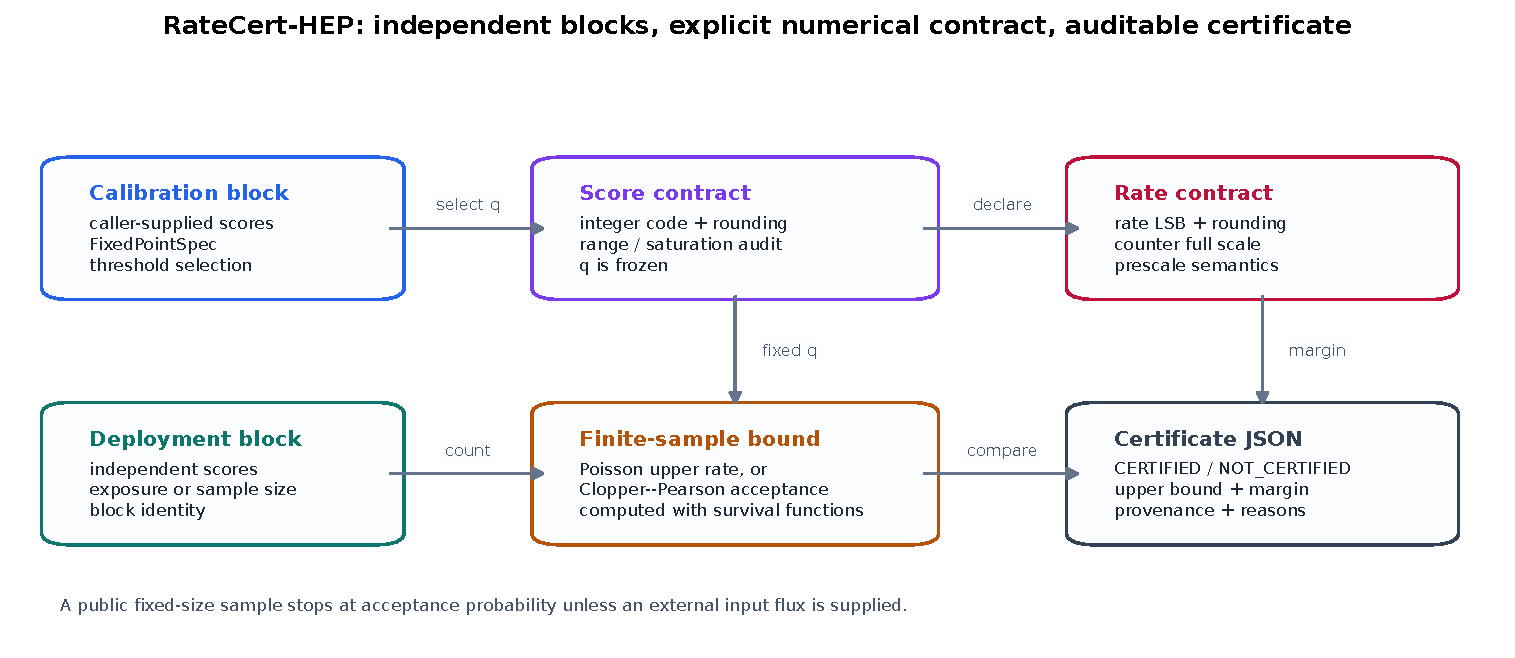
\includegraphics[width=\textwidth]{ratecert_architecture}
\caption{RateCert-HEP data flow.  Threshold selection consumes the calibration
block only; the deployment block is evaluated after the threshold is frozen.
The finite-sample and rate-register checks meet in the certificate, while a
public fixed-size sample stops at an acceptance probability unless an external
input flux is supplied.}
\label{fig:architecture}
\end{figure}

\subsection{Algorithms}

Algorithm~\ref{alg:certify} states the two-call interface that every evidence
chain in Sec.~\ref{sec:validation} uses: a calibration call that freezes an
integer threshold, and a deployment call that certifies it on independent
evidence.  The separation is structural, not conventional --- the deployment
call receives a threshold code and never the calibration array, so a caller
cannot accidentally re-certify the block that selected the threshold.

\begin{table}[t]
\centering\small
\caption{Threshold selection on the calibration block and certification on the
deployment block.  The two blocks must be disjoint; a call that presents the
same block identity twice is refused.}
\label{alg:certify}
\begin{tabular}{@{}p{0.94\textwidth}@{}}
\toprule
\textbf{Algorithm 1:} certify a fixed-point threshold \\
\midrule
\textbf{Input:} calibration scores $C$; deployment scores $D$; exposure $T$ or
sample size $n$; fixed-point spec $(b,f)$; rate spec $(\Delta_r,B,P)$; budget
$R_\mathrm{budget}$ or acceptance target $p_\mathrm{target}$; confidence
$\alpha$; block ids \\
\textbf{Output:} certificate with status, bound, margin, provenance, reasons \\
\midrule
1\ \ $\mathrm{id}_C \gets$ hash of calibration block identifier \\
2\ \ $\mathrm{id}_D \gets$ hash of deployment block identifier \\
3\ \ \textbf{if} $\mathrm{id}_C = \mathrm{id}_D$ \textbf{then return}
NOT\_CERTIFIED (\textit{calibration/deployment overlap}) \\
4\ \ $c \gets Q_b(C)$ \quad (\textit{vectorized fixed-point codes}, $O(n)$) \\
5\ \ \textbf{if} any code saturated \textbf{then} record saturation count \\
6\ \ $u \gets \mathrm{unique}(c)$; $r \gets$ reverse cumulative count of $u$
\quad (\textit{attainable curve}, $O(n\log n)$) \\
7\ \ $q \gets \arg\min_{q'\in u}$ having
$\mathrm{Upper}(r(q'),n,\alpha) < p_\mathrm{target}$ or
$\mathrm{Upper}(r(q'),T,\alpha)+\delta_r \le R_\mathrm{budget}$ \\
8\ \ \textbf{if} no such $q'$ \textbf{then return} NOT\_CERTIFIED
(\textit{target unreachable at this $\alpha$}) \\
9\ \ $K \gets \#\{d \in Q_b(D) : d \ge q\}$
\quad (\textit{deployment count, threshold frozen}) \\
10\ \ $U \gets$ Upper$(K, n$ or $T, \alpha)$
\quad (\textit{Eq.~\eqref{eq:poisson} or Eq.~\eqref{eq:binomial}}) \\
11\ \ $\delta_r \gets \Delta_r/2$ \textbf{if} nearest-even \textbf{else}
$\Delta_r$ \\
12\ \ \textbf{if} $(2^B-1)\Delta_r < U$ \textbf{then} reason $\gets$ counter
full scale \\
13\ \ \textbf{if} $U+\delta_r > R_\mathrm{budget}$ \textbf{then} reason $\gets$
budget margin \\
14\ \ \textbf{if} observed count overflows $B$ bits \textbf{then} reason $\gets$
count overflow \\
15\ \ \textbf{return} $U$, $\delta_r$, provenance, reasons, and status \\
\bottomrule
\end{tabular}
\end{table}

Algorithm~\ref{alg:baseline} states the four bound constructions compared in
Sec.~\ref{sec:baseline}.  Line 1 is the practice the paper argues against: it
returns the empirical tail, which is a point estimate and carries no coverage
guarantee.

\begin{table}[t]
\centering\small
\caption{The four upper-bound constructions evaluated on identical deployment
counts.  Only line 4 inverts an exact discrete sampling tail.}
\label{alg:baseline}
\begin{tabular}{@{}p{0.94\textwidth}@{}}
\toprule
\textbf{Algorithm 2:} upper bound $\mathrm{Upper}(K,n,\alpha)$ \\
\midrule
1\ \ \textbf{empirical:} \textbf{return} $K/n$ \\
2\ \ \textbf{Wald:} \textbf{return} $\hat p + z_{1-\alpha}
\sqrt{\hat p (1-\hat p)/n}$, \ where $\hat p = K/n$ \\
3\ \ \textbf{Wilson:} \textbf{return}
$\big(\hat p + z^2/2n + z\sqrt{\hat p(1-\hat p)/n + z^2/4n^2}\big)/(1+z^2/n)$,
\ where $z = z_{1-\alpha}$ \\
4\ \ \textbf{exact:} \textbf{if} $K = n$ \textbf{return} $1$
\quad (\textit{the incomplete beta degenerates here}) \\
\hspace*{2.2em} \textbf{else return}
$\mathrm{Beta}^{-1}(1-\alpha; K+1, n-K)$ \\
\bottomrule
\end{tabular}
\end{table}

\subsection{Computational complexity}

For a score array of length $n$, fixed-point conversion is a vectorized pass
with $O(n)$ time and memory.  The attainable threshold curve is constructed
from the $u$ distinct integer codes by a sorting-based unique operation and one
reverse cumulative sum; its worst-case cost is $O(n\log n)$ with $O(u)$
additional storage (and can be closer to linear when the implementation's
unique operation exploits bounded integer codes).  This cumulative construction
is important for dense score streams: a naive implementation that
rescans all $n$ values for every threshold has $O(nu)$ work.  Threshold selection
evaluates the candidate codes in ascending order and can make one beta-tail
call per candidate when calibration confidence is requested.  The final
certificate requires one count, one special-function evaluation, and constant
size metadata.

The quantization audit has two paths.  It uses a histogram and reverse
cumulative sum for quantized counts, then a sorted raw array for the descriptive
unquantized comparison.  Its memory use is linear in the supplied score stream;
the audit is therefore explicit and can be omitted in a latency-critical
caller while retaining the certificate contract.

\subsection{Certificate schema}

The JSON representation is intentionally flat at the top level so that a
workflow can filter results without importing Python.  Nested objects preserve
the exact numerical specifications.  Table~\ref{tab:schema} lists the fields
that determine interpretation.

\begin{table}[t]
\centering\small
\caption{Core fields in a RateCert-HEP certificate.}
\label{tab:schema}
\begin{tabular}{p{0.25\textwidth}p{0.64\textwidth}}
\toprule
Field & Meaning \\
\midrule
\texttt{status} & \texttt{CERTIFIED} or \texttt{NOT\_CERTIFIED}; the latter is a valid scientific result. \\
\texttt{count}, \texttt{sample\_size}, \texttt{exposure\_s} & Observed deployment evidence and its sampling semantics. \\
\texttt{upper\_acceptance}, \texttt{upper\_rate\_hz} & One-sided finite-sample bounds; absent rate fields mean no external flux was supplied. \\
\texttt{rate\_quantization} & LSB, rounding rule, counter bits, full scale, and deterministic margin. \\
\texttt{score\_quantization} & Score LSB, range, saturation count, and observed error diagnostics. \\
\texttt{deployment\_block\_id}, \texttt{calibration\_}\allowbreak\texttt{block\_id} & Evidence identities used to audit independence. \\
\texttt{provenance}, \texttt{warnings}, \texttt{reasons} & Source hashes, interpretation warnings, and every failed contract clause. \\
\bottomrule
\end{tabular}
\end{table}

\subsection{Numerical stability and boundary behavior}

The stringent family-wise corrections used in the scans can make $1-\alpha$
round to one in floating-point arithmetic.  The implementation therefore calls
the survival functions \texttt{chi2.isf} and \texttt{beta.isf}, rather than
forming an inverse CDF at $1-\alpha$.  The binomial routine returns one at the
$K=n$ boundary, and the Poisson routine accepts a zero count.  Empty or
non-finite score arrays are rejected before any division.  A saturated score is
retained by the diagnostic quantizer but fails strict certification because its
error is no longer bounded by an LSB.  These cases are covered by unit tests and
are visible in the JSON refusal path.

The LHCO adapter reads the released HDF5 feature table, selects only
\verb|label == 0| QCD background events, and derives the transparent scalar
$\sqrt{p_{x,j_1}^2+p_{y,j_1}^2}/5000\,\mathrm{GeV}$.  It records the source
DOI, license, file hashes, selection rule, split seed, and event-id hashes.
No generator, training procedure, or detector calibration is run during data
loading.

The quantization audit compares the quantized rule $Q_b(S)\ge q$ with the
descriptive unquantized rule $S\ge q\Delta_s$ for every observed code
threshold.  The maximum absolute difference is reported as a diagnostic.  It
is intentionally not added to Eq.~\eqref{eq:binomial} or Eq.~\eqref{eq:poisson}:
without a distributional assumption, a score LSB does not imply a universal
probability or rate change.

\subsection{Restrictions and non-goals}

The program does not train a classifier, choose a physics observable, estimate
a detector cross section, or synthesize an FPGA.  It does not infer live time
from the number of rows in a Monte Carlo file.  These exclusions keep the
scientific claim narrow enough to audit, and they are what allow a later
firmware or detector integration to supply its own score and input-flux
adapters without reopening the statistical argument.

% ---------------------------------------------------------------------------
\section{Validation protocol}
\label{sec:validation}

\subsection{Public LHCO sample}

The first experiment uses the LHC Olympics 2020 R\&D feature release, which
contains one million QCD background and one hundred thousand signal events
generated with Pythia8 and Delphes~\cite{Kasieczka2021LHCO,LHCO2020RND,
Sjostrand2015Pythia,deFavereau2014Delphes}.  The release has a high-$p_T$ event
selection and supplies no detector live time or representative input crossing
flux.  It is therefore used only for a background-acceptance experiment.

One hundred thousand background events are assigned to calibration and a
disjoint one hundred thousand to deployment by seed 20260912.  The sweep has
three score widths (8, 10, and 12 bits; the fractional-bit count equals the
total width in each unsigned format), three deployment prefixes (10,000,
50,000, and 100,000), and three
acceptance targets (0.5\%, 1\%, and 2\%).  The family-wise error probability is
1\%, giving $\alpha_{\rm cell}=0.01/27=0.0003703703704$.  Thresholds are chosen
with the calibration upper bound at this per-cell alpha and certified on the
independent deployment prefix.  The adapter verifies that the two selected
event-ID sets have empty intersection and records the seeded permutation split,
the two ID hashes, and the statement that statistical independence remains a
caller/data assumption rather than a proof supplied by the adapter.

\subsection{Explicit-exposure rate sample}

The second experiment isolates rate semantics with a declared Poisson
background rate of \SI{8}{Hz}.  It scans exposures of 1, 10, and 100 s, rate
LSBs of 0.01, 0.05, and \SI{0.1}{Hz}, unsigned counters of 8 and 16 bits, and
raw-rate budgets of 10 and \SI{12}{Hz}.  The 36 cells share a family-wise
alpha of 1\% ($\alpha_{\rm cell}=0.01/36$).  Each observed count is fed through
the same production certificate path with a binary score stream and prescale
$P=4$; the threshold is fixed at code one, so this benchmark tests the rate
contract without adding a second adaptive selector.  A separate 5,000-repeat
diagnostic at each exposure evaluates the Poisson upper-limit coverage at the
same per-cell alpha.

This second chain is deliberately synthetic, and that is the correct
instrument for the property it tests.  A coverage claim states that an interval
procedure contains the true rate in at least $1-\alpha$ of repetitions.  On a
real detector stream the true rate is unknown, so coverage is not observable;
only a generator with a declared ground-truth rate can measure it.  What the
synthetic chain cannot establish is detector stationarity, and the program
therefore refuses rather than assumes it (Sec.~\ref{sec:boundary}).

\subsection{Assumption-boundary stress}
\label{sec:boundary}

To expose rather than hide the sampling assumption, we run a separate
50,000-repeat diagnostic at a 10 s exposure and an 8 Hz mean rate.  The
stationary reference uses a Poisson count.  Two additional rows keep the same
nominal mean but use a two-state 0/40 Hz burst process and a gamma-mixed
window rate.  The latter rows deliberately violate the fixed-rate Poisson
model; their low coverage is a negative boundary result and is not folded into
the certified 36-cell sweep.

\subsection{Implementation and replay checks}

The validation suite tests the elementary numerical primitives and the higher
level refusal boundary.  It covers nearest-even and one-sided rounding,
saturation, zero-count Poisson limits, the counter-window conversion, full-scale
overflow, calibration/deployment identity overlap, JSON round trips, public
HDF5 selection, and the explicit acceptance and rate certificates.  The suite
is deliberately not a mirror of the implementation: each test asserts a
scientific invariant such as an upper bound above the point estimate, a
non-empty reason list on refusal, or exact preservation of the raw/recorded
prescale distinction.

Every benchmark cell is replayable from a recorded seed.  The public-data
adapter hashes the complete input file and hashes the selected event IDs for
both blocks.  The explicit-rate benchmark records the generated count, the
declared exposure, the true simulation rate used only for the coverage
diagnostic, and the full fixed-point specification.  Re-running a cell can
therefore distinguish a changed input or seed from a changed implementation.
The helper \path{make_replay_table.py} flattens all 27 public and 36 explicit
cells into a CSV containing the parameters, bounds, margins, status, and refusal
reasons used for the headline counts.

\subsection{Reference-platform timing}

We include a timing diagnostic to expose the cost of the Python reference
implementation without presenting it as detector latency.  On an Intel
Core i7-10750H laptop (6 physical cores, Python 3.10.7, NumPy 1.26.4, SciPy
1.15.3), 20 median timings were collected for a 100,000-event array.  The
vectorized score quantizer took 2.37 ms, the public acceptance certificate
2.81 ms, and the explicit rate certificate 7.20 ms.  The latter includes the
attainable threshold curve and its cumulative-code implementation.  These
figures are reference-platform throughput measurements; firmware clocking,
memory layout, detector deadtime, and trigger latency remain outside the
scope of this release.

% ---------------------------------------------------------------------------
\section{Results}
\label{sec:results}

\begin{figure}[t]
\centering
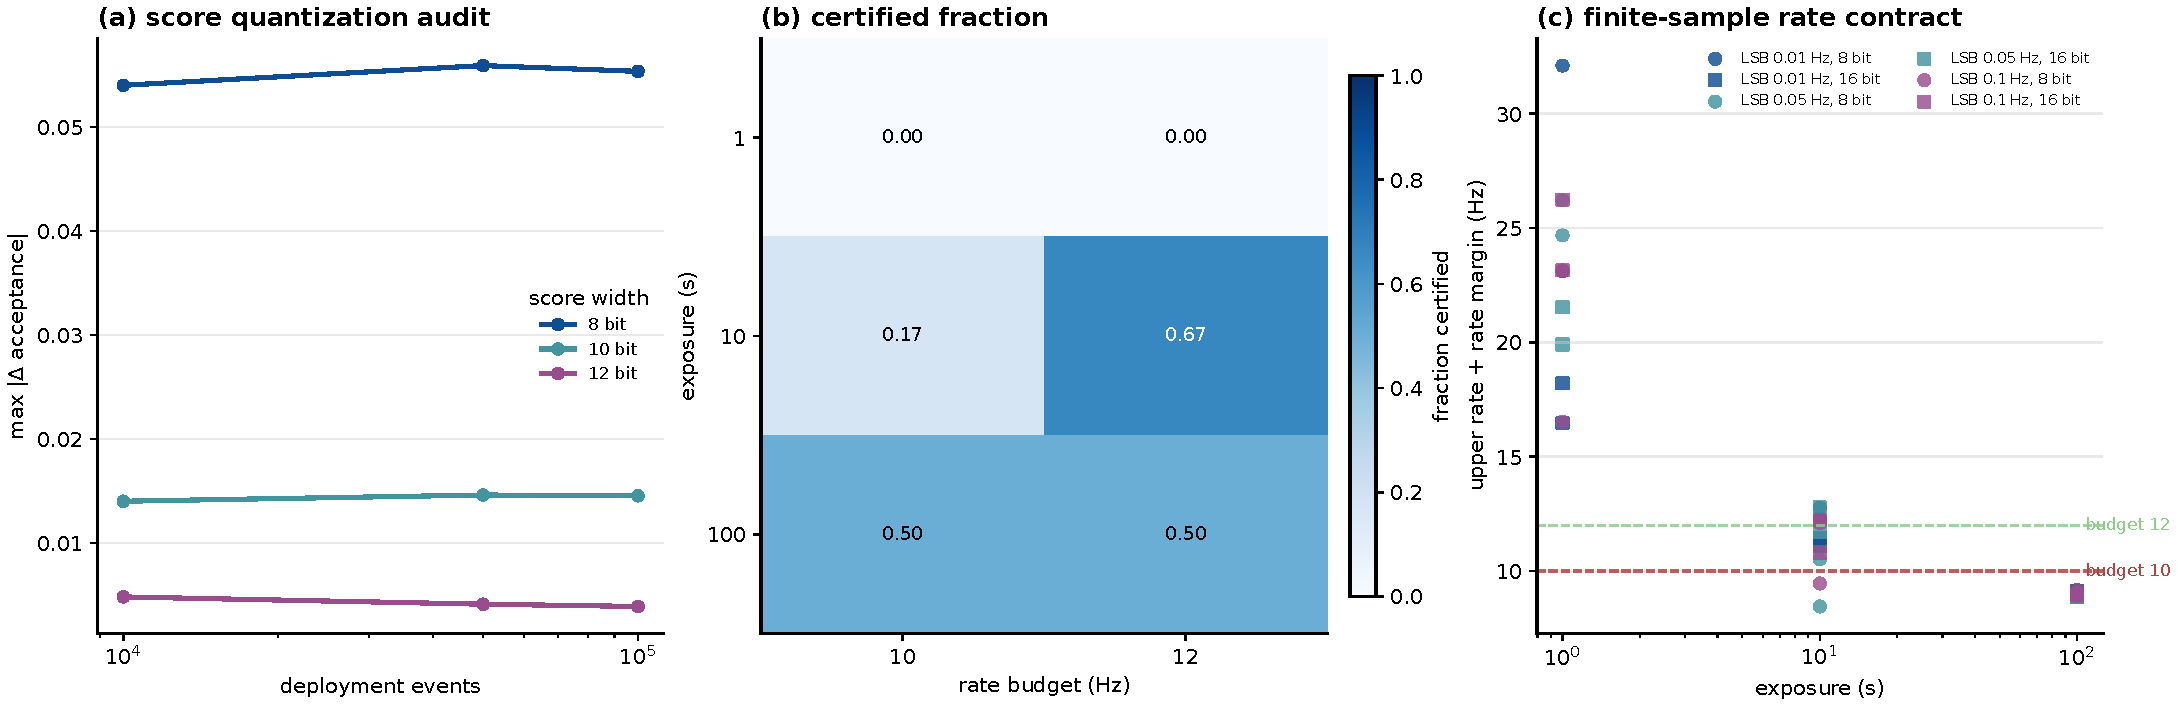
\includegraphics[width=\textwidth]{unified_benchmark}
\caption{Unified RateCert-HEP validation.  (a) Maximum observed acceptance
change caused by score quantization, evaluated over every observed code
threshold.  (b) Fraction of explicit-rate cells certified after aggregation
over rate LSB and counter width.  (c) One-sided upper rate plus the declared
rate-register margin; dashed lines are the raw-rate budgets.  The LHCO panel
uses acceptance probability, whereas the rate panels use declared Poisson
exposures.}
\label{fig:unified}
\end{figure}

\subsection{Acceptance and quantization}

The public experiment certifies 19 of 27 cells.  The eight refusals occur when
the independent finite-sample upper acceptance remains above the requested
target, primarily for the 0.5\% target at smaller prefixes.  The result is
expected: increasing the number of events tightens the upper limit, while the
certificate does not relax its confidence requirement to preserve a high pass
rate.

The all-threshold quantization audit finds maximum absolute acceptance changes
of 0.0559, 0.0146, and 0.0048 for 8, 10, and 12 bits, respectively.  At the
selected high-tail thresholds the corresponding signed diagnostic is often much
smaller, because the released feature values leave few events in the half-LSB
boundary interval.  Both facts are retained: the former warns about potential
boundary aliasing, and the latter describes the operating point without turning
it into a distribution-free guarantee.

The independent 20,000-repeat binomial coverage stress test gives coverages of
1.0000, 0.99965, 0.99965, and 0.99945 over its four sample-size and target
acceptance settings, against the nominal per-cell coverage 0.9996296.  This is
an implementation diagnostic rather than a replacement for the exact
Clopper--Pearson guarantee.  Figure~\ref{fig:acceptance} makes the acceptance
margin visible at the selected operating points: an open cross is a refusal
whose upper bound remains above the requested target.

\begin{figure}[t]
\centering
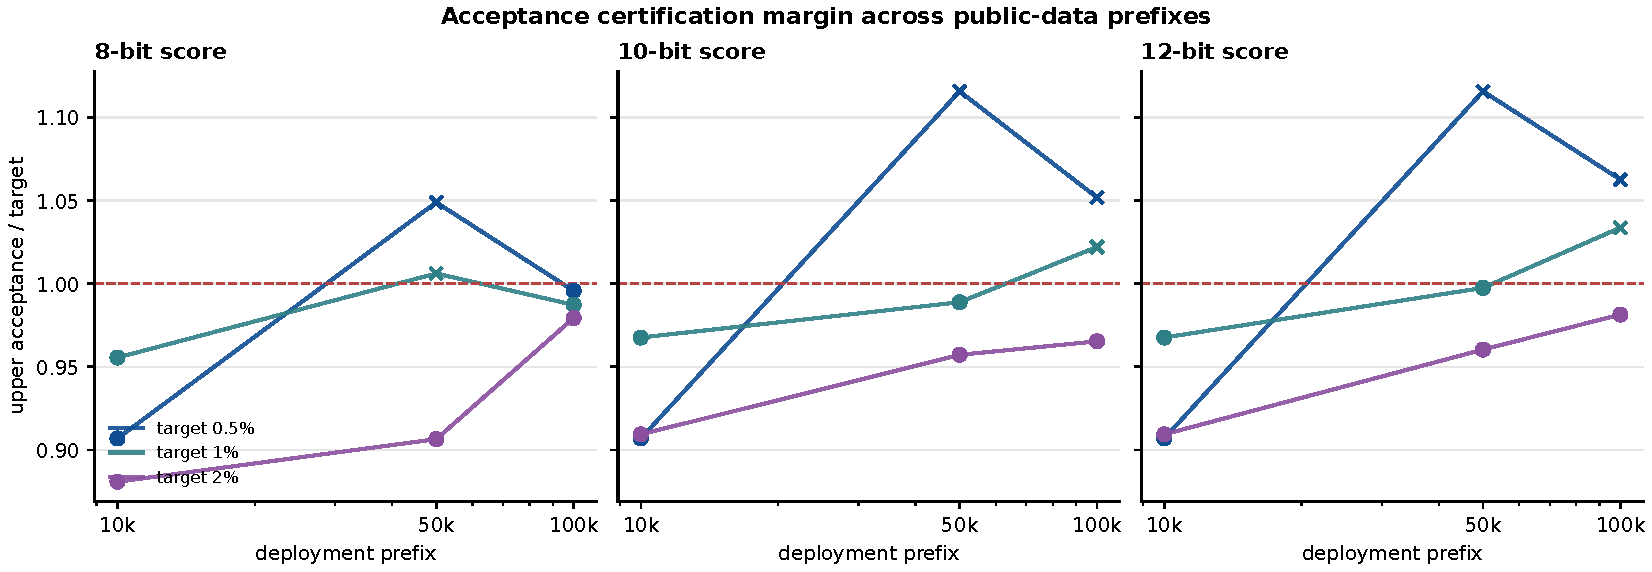
\includegraphics[width=\textwidth]{acceptance_certification}
\caption{Public LHCO acceptance margin.  Each point is the deployment
Clopper--Pearson upper acceptance divided by its requested target, plotted for
the three deployment prefixes and three score widths.  Filled circles are
certified cells; crosses are retained refusals.  The dashed line is the exact
pass boundary, so the figure exposes both statistical headroom and the effect
of finite prefixes.}
\label{fig:acceptance}
\end{figure}

\subsection{Explicit rate and coverage}

The explicit-exposure benchmark certifies 11 of 36 cells.  One-second cells
often fail because the confidence upper bound is too wide for a 10--12 Hz
budget.  Eight-bit counters fail at 100 s because their full scale is below the
approximately 8 Hz rate when the declared LSB is 0.01, 0.05, or 0.1 Hz.  These
are distinct refusal reasons in the JSON report.  The 1, 10, and 100 s
coverage diagnostics are 1.0000, 0.9998, and 0.9998, respectively, against the
nominal per-cell coverage 0.9997222.

The assumption-boundary stress makes the scope testable.  At $\alpha=0.01$,
the stationary reference covers 0.99108 of repeats, while the two-state burst
and gamma-mixed rows cover 0.19386 and 0.56002, respectively, despite having
the same nominal mean rate.  This is the expected failure mode when a production stream
violates the declared fixed-rate Poisson model; the software must refuse to
interpret these rows as certified rates.

\begin{figure}[t]
\centering
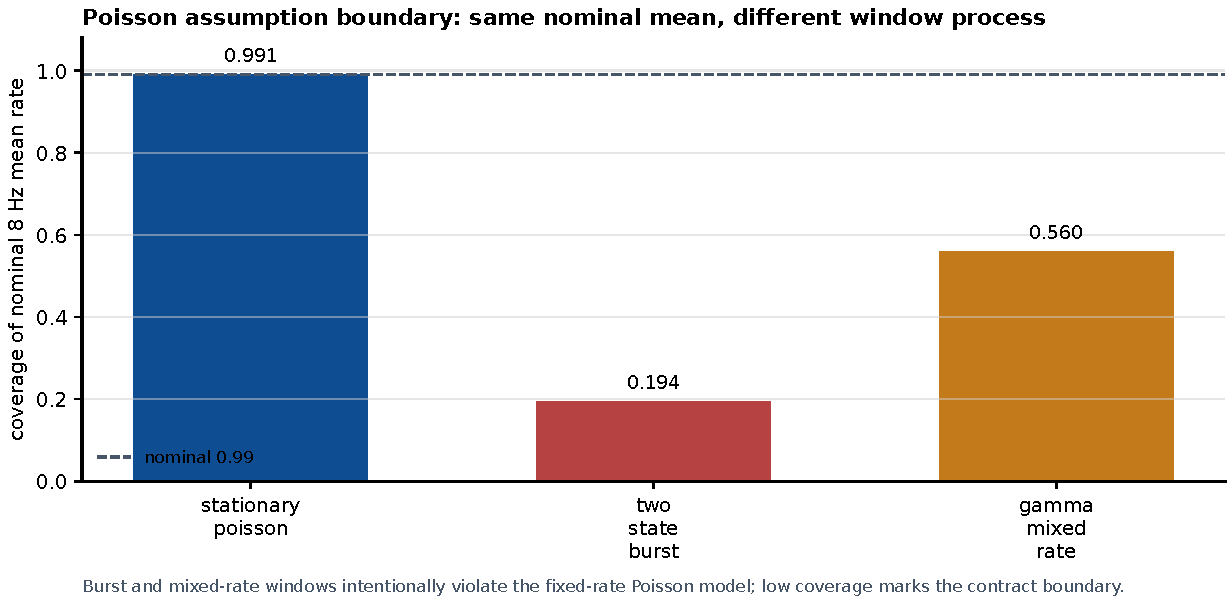
\includegraphics[width=0.86\textwidth]{assumption_boundary}
\caption{Poisson assumption boundary.  All rows have a nominal mean of 8 Hz
over a 10 s window, but only the first follows the stationary fixed-rate
Poisson model.  The burst and mixed-rate rows are deliberately misspecified;
their reduced coverage is retained as a failure diagnostic rather than hidden
behind the exact Poisson theorem.}
\label{fig:assumption}
\end{figure}

Figure~\ref{fig:coverage} reports both coverage diagnostics with their
Monte-Carlo repeat uncertainty.  The intervals quantify the variability of the
diagnostic itself; the finite-sample guarantees remain the exact tail
inversions in Eqs.~\eqref{eq:poisson} and~\eqref{eq:binomial}.

\begin{figure}[t]
\centering
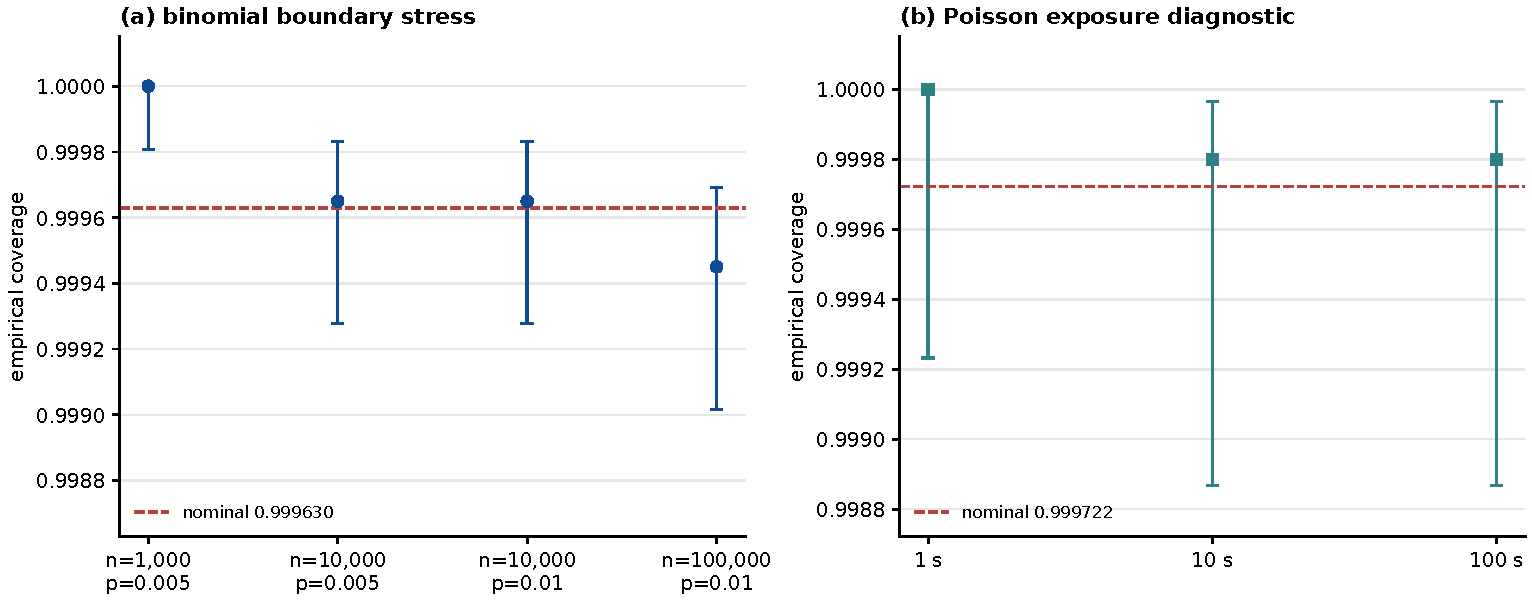
\includegraphics[width=\textwidth]{coverage_diagnostics}
\caption{Finite-sample coverage diagnostics.  (a) Binomial boundary stress
scenarios from the independent 20,000-repeat experiment.  (b) Poisson
coverage at 1, 10, and 100 s exposures.  Points are empirical coverage and
bars are 95\% repeat-level intervals; dashed lines are the nominal per-cell
coverage.  These are implementation diagnostics, not substitutes for the
exact Clopper--Pearson or Poisson bounds.}
\label{fig:coverage}
\end{figure}

\subsection{Quantitative comparison with alternative bounds}
\label{sec:baseline}

The preceding sections argue that an exact one-sided bound is the right
construction, but they do not show what the alternatives would have produced.
We therefore apply four upper-bound constructions to the \emph{identical} 27
deployment cells at the same per-cell $\alpha$; only the construction differs.
The four are the empirical tail reported as if it were a probability
($U=K/n$), a one-sided normal (Wald) bound, a one-sided Wilson score bound, and
the exact Clopper--Pearson bound of Eq.~\eqref{eq:binomial} used here.

\begin{table}[t]
\centering\small
\caption{The same 27 deployment cells certified under four upper-bound
constructions, at the identical per-cell $\alpha=0.01/27$.  A cell is certified
when its bound falls below the requested target.}
\label{tab:baseline}
\begin{tabular}{lr}
\toprule
Bound construction & Cells certified (of 27) \\
\midrule
Empirical tail $K/n$ (no uncertainty) & 27 \\
One-sided normal (Wald) bound & 20 \\
One-sided Wilson score bound & 18 \\
Exact Clopper--Pearson (this work) & 19 \\
\bottomrule
\end{tabular}
\end{table}

Table~\ref{tab:baseline} is the substance of the argument.  The empirical tail
certifies \emph{every} cell.  It does so not because every configuration is
safe but because it carries no uncertainty at all: at $n=10^4$ and a target of
0.5\% it returns an upper bound of 0.0024 where the exact construction returns
0.0045, roughly a factor of two optimism from a quantity that is supposed to be
a bound toward safety.  Reporting $K/n$ as an upper limit is therefore not a
conservative approximation; it is the removal of the guarantee.

Coverage against a known ground truth makes the consequence explicit.
Table~\ref{tab:coverage-baseline} draws binomial counts with a declared true
acceptance probability and measures how often each bound actually contains it,
at the per-cell $\alpha$ of the public sweep.

\begin{table}[t]
\centering\small
\caption{Empirical coverage of the true acceptance probability, nominal
coverage $0.9996296$, 20{,}000 repeats per setting.  A valid one-sided bound
must reach the nominal value; a value below it means operating points can be
certified that should not be.}
\label{tab:coverage-baseline}
\begin{tabular}{rrcccc}
\toprule
$n$ & true $p$ & Clopper--Pearson & Wilson & Normal & $K/n$ \\
\midrule
1{,}000   & 0.005 & 1.000000 & 1.000000 & 0.958500 & 0.559900 \\
10{,}000  & 0.005 & 0.999750 & 0.999950 & 0.997800 & 0.522150 \\
10{,}000  & 0.010 & 0.999750 & 0.999800 & 0.998950 & 0.509800 \\
100{,}000 & 0.010 & 0.999650 & 0.999700 & 0.999300 & 0.505350 \\
\bottomrule
\end{tabular}
\end{table}

Two results are worth stating precisely.  First, the empirical tail attains
about 0.51--0.56 coverage against a nominal $0.9996296$.  It is a point
estimate, so it covers only when the sample proportion happens to exceed the
true probability, and the certification it grants is not a statistical
statement at all.  Any workflow that treats a small empirical tail as a
certified rate inherits this failure mode, and the failure is silent: the
report looks like a pass.  Second, the one-sided normal bound under-covers at
the small counts that matter most here ($0.9585$ at $n=10^3$, $p=0.005$),
which is the known degeneracy of the Wald interval when $n\hat p$ is small ---
precisely the regime of a high-tail trigger threshold.  It nevertheless
certifies \emph{more} cells than the exact bound (20 against 19), which is
exactly backwards: the construction that fails to cover is the one that is more
permissive.  Figure~\ref{fig:baseline} shows both effects together.

\begin{figure}[t]
\centering
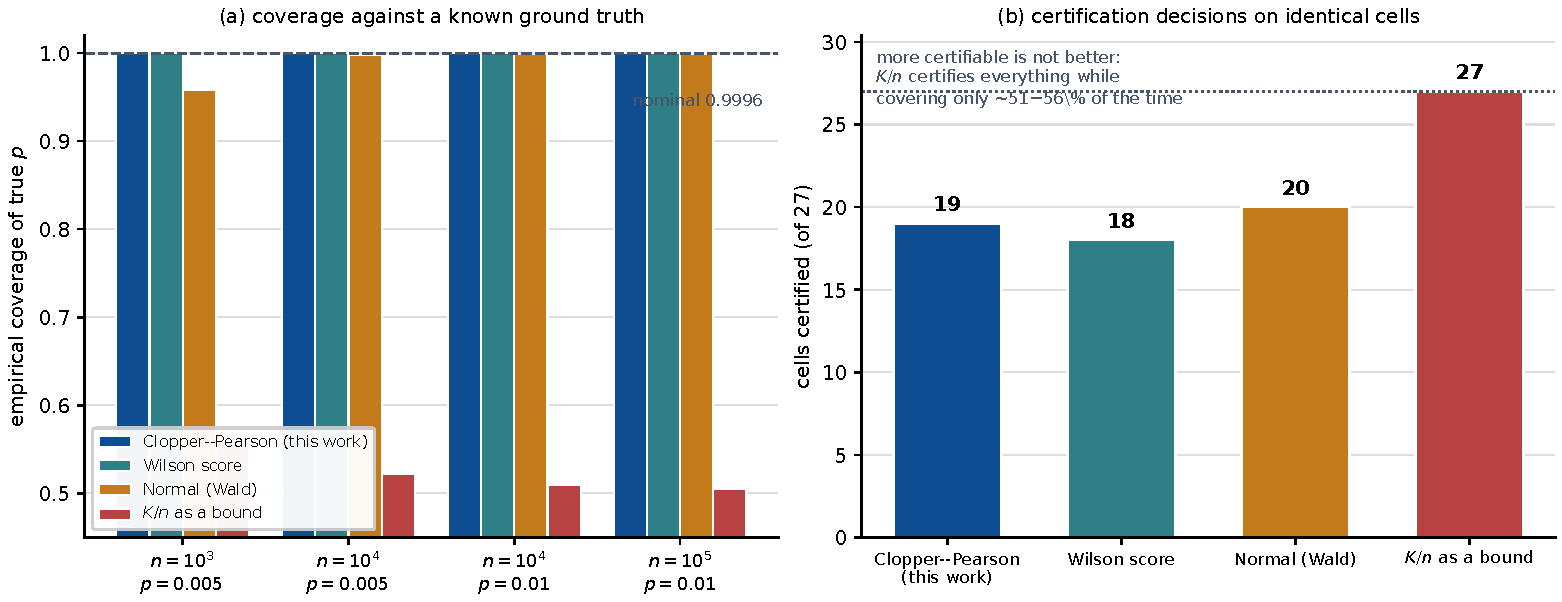
\includegraphics[width=\textwidth]{baseline_coverage}
\caption{Baseline comparison.  (a) Empirical coverage of the true acceptance
probability against the nominal $0.9996296$, 20{,}000 repeats per setting.  The
normal bound under-covers at small counts; the empirical tail covers roughly
half the time.  (b) Certification decisions of the four constructions on the
identical 27 deployment cells.  More certifiable is not better: the empirical
tail certifies every cell while providing no coverage guarantee.}
\label{fig:baseline}
\end{figure}

Wilson's interval tracks the exact bound closely in coverage and is the
strongest of the three alternatives; we do not claim otherwise.  The reason we
ship the exact construction rather than Wilson is not superior coverage but
non-negotiability.  Clopper--Pearson is an inversion of the exact discrete
sampling tail, so its coverage is guaranteed at every $(n,p)$ rather than
asymptotically, and the guarantee is what a rate-budget pass is supposed to
mean.  This is a deliberate choice against a well-documented body of advice:
Wilson and Agresti--Coull intervals are often recommended in preference to
``exact'' intervals because they are shorter at equal nominal coverage and
avoid the conservatism of the discrete inversion~\cite{Agresti1998,Brown2001}.
That trade is the right one for estimation, where a shorter interval is
strictly more informative.  It is the wrong trade for a pass/fail deployment
predicate, because there the interval is being used as a guarantee and the
cost of over-coverage is a refused configuration whereas the cost of
under-coverage is an unsafe one accepted.  The price is visible in
Table~\ref{tab:baseline}: two cells that Wilson would certify are refused here.
We regard refusing a marginal cell as the correct behaviour for a certification
tool, and the refusal is retained with its reason rather than dropped.  For the
same reason the Poisson path follows the classical
Garwood construction~\cite{Garwood1936} rather than a normal approximation.

\subsection{Evidence-chain summary}

Table~\ref{tab:results} summarizes the independent evidence chains.  The
public chain establishes that the same API can certify a fixed-size simulated
sample without fabricating a live rate.  The explicit chain exercises the
Poisson path, the rate-register margin, and the counter range.  The coverage
experiments are diagnostics of implementation behavior; the formal confidence
statements remain those in Eqs.~\eqref{eq:poisson} and~\eqref{eq:binomial}.

\begin{table}[t]
\centering\small
\caption{Evidence-chain results produced by the checked-in benchmark scripts.}
\label{tab:results}
\begin{tabular}{p{0.18\textwidth}p{0.06\textwidth}p{0.09\textwidth}p{0.07\textwidth}p{0.14\textwidth}p{0.18\textwidth}}
\toprule
Evidence chain & Cells & Certified & Ref. & Repeats & Primary output \\
\midrule
LHCO public acceptance & 27 & 19 & 8 & -- & $p$ upper bound \\
Explicit Poisson rate & 36 & 11 & 25 & 5,000 per exposure & raw Hz upper bound \\
Binomial coverage stress & 4 & -- & -- & 20,000 per cell & 0.99945--1.00000 \\
\bottomrule
\end{tabular}
\end{table}

\subsection{Refusal taxonomy}

The negative results are not a single catch-all.  In the public sweep, eight
cells fail because the deployment Clopper--Pearson upper acceptance remains
above the requested target.  In the explicit sweep, 19 cells fail the budget
after adding the rate-register margin, eight exceed the declared counter
full-scale upper rate, and six also encounter an observed-count overflow in the
8-bit counter.  These categories overlap, so their counts are intentionally not
added to obtain 25.  Keeping the predicates separate makes it possible to tell
whether more exposure, a wider counter, or a different budget would address a
failure.

Figure~\ref{fig:refusal} separates the exposure trend in these predicates.
The one-second configuration is dominated by the budget margin, whereas the
100-second configuration exposes the finite counter range and count overflow.

\begin{figure}[t]
\centering
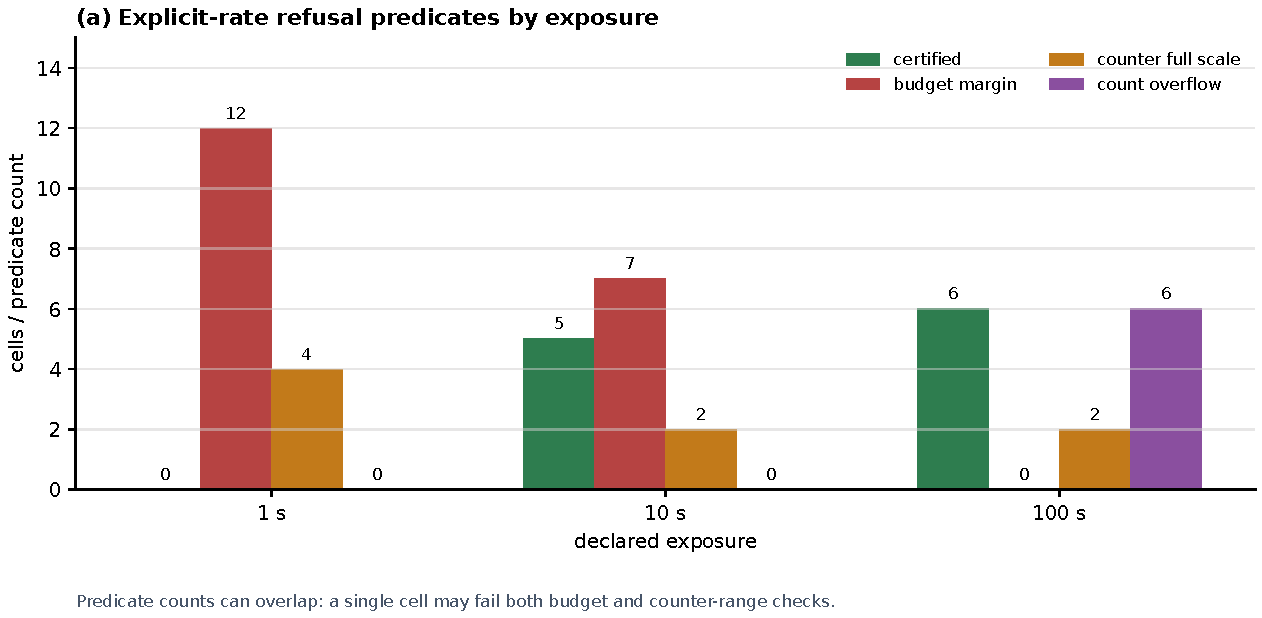
\includegraphics[width=0.86\textwidth]{refusal_taxonomy}
\caption{Explicit-rate refusal taxonomy by declared exposure.  Bars count
certified cells and the occurrence of each refusal predicate across the 12
cells at an exposure.  Predicate counts intentionally overlap: a cell can
fail both the budget-margin and counter-range clauses, so the bars are a
diagnostic of failure modes rather than a partition of the 36 cells.}
\label{fig:refusal}
\end{figure}

\subsection{Timing result and algorithmic effect}

The cumulative-code construction in \texttt{rate\_curve} changes the reference
certificate timing for 100,000 events from a repeated full-array scan to a
single unique-and-cumulative pass.  On the reference platform the median
timings are 2.37 ms for quantization, 2.81 ms for the public acceptance
certificate, and 7.20 ms for the explicit rate certificate over 20 repeats.
These numbers are included to make scaling behavior inspectable, not to imply
that Python is a trigger implementation or that the statistic can be evaluated
inside a detector clock cycle.

% ---------------------------------------------------------------------------
\section{Reproducibility and failure semantics}
\label{sec:repro}

The source tree contains the data adapter, configuration examples, test
suite, benchmark scripts, reports, and figure manifest.  A clean run is:

\begin{verbatim}
py -m pip install -e ".[dev,public-data,figures]"
$env:PYTHONPATH = "src"
$dataset = "data/public/lhco_rnd/"
$dataset += "events_anomalydetection_v2.features.full.h5"
py examples/unified_benchmark.py `
  --public-input $dataset `
  --output reports/unified_benchmark.json
py examples/make_unified_figure.py `
  --input reports/unified_benchmark.json `
  --output-stem reports/figures/unified_benchmark
py examples/make_architecture_figure.py `
  --output-stem reports/figures/ratecert_architecture
py examples/make_diagnostic_figures.py `
  --unified reports/unified_benchmark.json `
  --coverage reports/coverage_stress.json `
  --output-dir reports/figures
py examples/assumption_boundary_stress.py `
  --output reports/assumption_boundary_stress.json
py examples/make_replay_table.py `
  --input reports/unified_benchmark.json `
  --output reports/reviewer_replay_table.csv
py examples/performance_benchmark.py
py -m pytest tests -q
\end{verbatim}

\subsection{Worked API path}

The minimal synthetic example uses the same two calls as the public and
explicit benchmarks.  The first call freezes a threshold from calibration; the
second call evaluates an independent deployment array.  A caller that already
has a firmware threshold can skip selection and pass that integer directly.

\begin{verbatim}
score_spec = FixedPointSpec(bits=10, fractional_bits=8)
rate_spec = RateQuantizationSpec(lsb_hz=0.05, counter_bits=32)
decision = choose_threshold(calibration_scores,
                            exposure_s=20.0,
                            target_rate_hz=8.0,
                            spec=score_spec)
certificate = certify_rate(
    deployment_scores, exposure_s=20.0,
    threshold_code=decision.threshold_code,
    rate_budget_hz=12.0, alpha=0.01,
    spec=score_spec, rate_spec=rate_spec,
    deployment_block_id="synthetic-deploy-v1",
    calibration_block_id="synthetic-cal-v1", prescale=4)
write_json("reports/certificate.json", certificate.as_dict())
\end{verbatim}

The public-data path replaces the first two lines with the LHCO loader, passes
the calibration scores to the acceptance-threshold selector, and passes the
deployment scores to the acceptance certifier.  The resulting object labels
its quantity as a background acceptance probability and leaves the absolute-rate
fields empty until an external input flux, budget, and rate specification are
provided together.

\subsection{Worked example with checked-in expected output}
\label{sec:worked}

The distribution contains a self-contained test run that requires no external
data, together with the exact output it must produce.  The input is a
deterministic 16{,}000-event score stream generated at seed 20260912; the
fixed-point specification is 10 bits with 8 fractional bits, so the score LSB is
$2^{-8}$ and integer code $q$ corresponds to score $q/256$.  The declared rate
register has a 0.05 Hz LSB with nearest-even rounding, a prescale of 4, and a
32-bit counter; the budget is 12 Hz at $\alpha=0.01$ over a 20 s exposure.

At threshold code 250 the deployment block returns $K=145$, and the certificate
contains
\begin{center}\small
\begin{tabular}{@{}lr@{}}
\toprule
Field & Value \\
\midrule
\texttt{threshold\_code} & 250 \\
\texttt{count} & 145 \\
\texttt{point\_rate\_hz} & 7.25 \\
\texttt{upper\_rate\_hz} & 8.778530889551678 \\
\texttt{quantization\_margin\_hz} & 0.025 \\
\texttt{deployment\_margin\_hz} & 3.1964691104483216 \\
\texttt{recorded\_point\_rate\_hz} & 1.8125 \\
\texttt{saturation\_count} & 0 \\
\bottomrule
\end{tabular}
\end{center}
The decision illustrates the point of the contract.  The point estimate
$7.25$~Hz is not the certified quantity.  The pass predicate evaluates
$8.778530889551678 + 0.025 = 8.80353 \le 12$, so the configuration is certified
with a remaining margin of $3.1965$~Hz.  The recorded rate is reported
separately as $1.8125$~Hz for $P=4$ and does not enter the predicate, since a
prescale does not reduce the raw rate the budget constrains.

Moving the threshold by one code to 249 raises the count to 205 and the upper
rate to $12.04261$~Hz.  The predicate then gives
$12.04261 + 0.025 = 12.06761 > 12$, and the configuration is refused by
$0.068$~Hz with the single reason
\textit{finite-sample upper rate plus fixed-point margin exceeds budget}.  The
refusal is returned as a valid structured object, not as an error.  A third
case keeps code 250 but declares a 4-bit counter, whose full scale is
$(2^4-1)\times0.05 = 0.75$~Hz.  It is refused with two independent reasons,
\textit{rate counter overflow: count 145 exceeds 15} and \textit{finite-sample
upper rate exceeds the declared rate-counter full scale}; the predicates are
reported separately because they call for different remedies.  All three runs
use the same code path, so a reviewer can confirm that only the statistical
bound and the register margin enter the pass condition.

\subsection{Reproducibility contract}

The repository stores configuration, source scripts, reports, and figure
manifests as ordinary text or binary artifacts.  Each report includes the seed,
cell parameters, and interpretation boundary.  The public report additionally
stores the complete input-file hash and event-ID hashes for both blocks.  The
figure manifest stores the hash of the JSON input used to draw it.  This
file-level chain does not attempt to prove the provenance of an external
detector stream; it makes the provenance of the supplied evidence explicit.

The package is installable in editable mode with the optional extras shown
above.  The reference versions used for the reported replay are pinned in
\path{requirements-lock.txt}.  The core path depends only on NumPy and SciPy;
pandas/PyTables are needed for the HDF5 adapter and Matplotlib only for the
paper figures.  A user
who does not have the public file can still run the synthetic certificate and
all core tests, while the public-data result is correctly unavailable rather
than silently replaced by synthetic rows.

The current run produces 30 passing tests, the 27-cell public report, and the
36-cell explicit-rate report.  It also produces the architecture diagram,
three diagnostic figures plus the assumption-boundary stress figure (each in
300 dpi PNG and vector PDF form), a reviewer replay table, a timing report,
and manifests with the input-report hashes.  The downloaded
LHCO feature file is identified by the
following provenance values:
\begin{center}\small
DOI: \verb|10.5281/zenodo.6466204|\\
MD5: \verb|271cf5e71fc756b2a8d2b32730689bdb|\\
SHA-256: \texttt{933b1f11d7b66e6d}\allowbreak
\texttt{ae0ee2878723f8f5d7ab0f38399806f2d067c5cfd9a502b1}
\end{center}

Scientific refusals return a valid JSON certificate with status
\verb|NOT_CERTIFIED| and a non-empty reason list.  Malformed files or configurations
return a command-line error.  This separation lets automated campaigns retain
negative evidence instead of silently dropping difficult operating points.

% ---------------------------------------------------------------------------
\section{Discussion and limitations}
\label{sec:discussion}

The main validity condition is independence between calibration and deployment
blocks, together with a stable deployed score definition.  A public simulation
sample can test the software and its statistical accounting, but it cannot
establish detector stationarity, trigger latency, or a physical crossing flux.
The LHCO data are also selected and simulated, so their acceptance distribution
should not be read as a CMS or ATLAS background rate.

The quantization audit is deliberately descriptive.  A universal bound on the
acceptance change caused by a score LSB would require additional assumptions,
such as a bounded density near every threshold.  Likewise, a rate-register LSB
is a numerical representation margin; it does not bound the change in rate
caused by changing the score threshold.  RateCert-HEP keeps these claims
separate so that a future hardware integration can add a measured live-time and
input-flux contract without changing the finite-sample theorem.

The present release is a reference implementation rather than a synthesized
FPGA design.  It does not measure latency, resource use, or detector deadtime.
Its value is the executable refusal boundary and the reproducible evidence
record: a configuration passes only when the statistical upper limit, the
declared rate representation, the counter range, and all provenance checks
agree.

\subsection{Position relative to existing statistical software}

Prior limit-setting programs in this journal, POLE 1.0~\cite{Conrad2004POLE}
and TRolke 2.0~\cite{Lundberg2010TRolke}, established that exact one-sided
Poisson intervals, including systematic uncertainties, can be delivered as
reusable software, and the Bayesian analysis toolkit~\cite{BAT2009} extended
that treatment to a full posterior.  RateCert-HEP does not repeat that work:
it evaluates the same class of exact one-sided limits, and it does so through
survival functions rather than inverse-CDF evaluation, but the statistical
content is not its contribution.

The difference is what the returned number is attached to.  A limit-setting
program takes a count and an exposure and returns an interval; the provenance
of the count, the identity of the sample on which the threshold was selected,
and the representation of the result in firmware are all outside its scope.  In
a trigger deployment those are precisely the quantities that can invalidate an
apparently safe menu entry: a threshold chosen on the same events that certify
it, or a rate register too narrow to hold the certified upper limit, produces a
number that is arithmetically correct and operationally wrong.  RateCert-HEP
certifies the composition, and refuses when the composition cannot be
supported.

YODA demonstrates how a mature HEP library can make statistical objects
consistent across aggregation, persistence, and plotting~\cite{YODA}.  Its
histograms and profiles are natural consumers of trigger streams, but they do
not constitute a deployment certificate: a histogram does not decide whether a
threshold was selected independently, whether an exposure is known, or whether
a rate register has enough range.  RateCert-HEP occupies this narrower control
plane.  It can consume a caller's score stream before or after a histogramming
workflow, and it emits a machine-readable decision that a batch system can
archive beside the analysis products.

The distinction is summarized below.

\begin{table}[t]
\centering\small
\caption{Scope comparison with a general HEP statistical utility.}
\label{tab:scope}
\begin{tabular}{p{0.28\textwidth}p{0.29\textwidth}p{0.29\textwidth}}
\toprule
Capability & General histogramming workflow & RateCert-HEP \\
\midrule
Primary object & Binned moments, profiles, and plots & Threshold certificate with an upper bound and margin \\
Evidence semantics & Aggregates fills, optionally with weights & Requires separate calibration/deployment identities \\
Rate interpretation & Depends on caller's normalization & Declares exposure or refuses absolute Hz \\
Finite-sample decision & Usually a reported uncertainty & Exact one-sided Poisson or binomial pass condition \\
Fixed-point deployment & Representation of stored values & Score and rate register contracts, range, and saturation refusal \\
Negative evidence & Workflow-specific & Structured \texttt{NOT\_CERTIFIED} reasons \\
\bottomrule
\end{tabular}
\end{table}

\subsection{Threats to validity and extension path}

The theorem assumes that the deployment events obey the declared sampling model
and that the score implementation is stable between calibration and
deployment.  A block ID is evidence for bookkeeping, not a cryptographic proof
that two arrays were generated independently; a production integration should
add run IDs, configuration digests, and an acquisition-level split guarantee.
The current adapter also treats events as unweighted Bernoulli trials.  Weighted
Monte Carlo, time-dependent backgrounds, and correlated bursts require an
explicit effective-sample or point-process model before they can be certified.

The extension path is intentionally local.  A hardware adapter would supply a
measured live-time interval, an input crossing flux, the firmware score-code
equivalence test, and the exact register specification.  Those additions would
populate existing fields such as $T$, $p_{\rm input}$, and $\Delta_r$; they do
not require changing the adaptive-threshold argument.  A future streaming
adapter can reuse the cumulative-code and JSON layers while replacing the
independent-block assumption with a declared sequential confidence procedure.

The distributed release includes a compact verification checklist: install the
core extra, run the synthetic certificate, run the 30-test suite, replay the
public-data command when the 74 MB file is available, inspect the JSON refusal
reasons, and regenerate both figure formats.  Each step has a checked-in input
or a precise external-data hash, so a failure can be localized to dependencies,
data provenance, numerical code, or a changed scientific result.  A referee can
therefore build, run, and audit the program without access to any internal data.
The release is archived at \url{https://github.com/pixele8/ratecert-hep} under
the MIT licence, tagged \texttt{v0.1.0}.

% ---------------------------------------------------------------------------
\section{Conclusion}
\label{sec:conclusion}

RateCert-HEP turns a commonly implicit trigger-rate argument into an executable
contract.  It separates score quantization from rate-register resolution,
selects thresholds on independent blocks, uses exact one-sided finite-sample
limits, and preserves negative results.  The public LHCO experiment verifies
the acceptance-probability path, while the explicit Poisson sweep verifies the
rate and resolution path.  Together they provide a reproducible baseline for
future firmware and live-detector integration, with the assumptions and
boundaries exposed for review.

% ---------------------------------------------------------------------------
\appendix

\section{Derivation of the one-sided limits}
\label{app:limits}

For the Poisson path write $\mu=\lambda T$.  The probability of observing no
more than $N$ events is the Poisson lower tail, which is monotone decreasing in
$\mu$.  Inverting this tail at $\alpha$ gives the unique $\mu_+$ satisfying
\begin{equation}
 \Pr_{\mu_+}(X\le N)=\alpha,
 \qquad X\sim\operatorname{Poisson}(\mu_+).
 \label{eq:poisson-inversion}
\end{equation}
The Poisson--chi-square identity converts this solution to
$2\mu_+=\chi^2_{1-\alpha,2(N+1)}$, which is Eq.~\eqref{eq:poisson} after
division by $T$.  The inversion is monotone, so observing a count whose true
mean is above the returned limit has probability at most $\alpha$.

For the fixed-size path, the event count is $K\sim\operatorname{Binomial}(n,p)$.
The upper limit is obtained by solving
\begin{equation}
 \Pr_{p_+}(K'\le K)=\alpha,
 \qquad K'\sim\operatorname{Binomial}(n,p_+).
 \label{eq:binomial-inversion}
\end{equation}
The beta--binomial identity gives
$p_+=\operatorname{Beta}^{-1}(1-\alpha;K+1,n-K)$ for $0\le K<n$.  At the
boundary $K=n$ the second shape parameter $n-K$ vanishes and the incomplete
beta function is not defined, so the implementation assigns $p_+=1$ directly
rather than evaluating the identity.  Both limits are therefore inversions of
exact discrete sampling tails rather than normal approximations.  The
survival-function calls in the implementation evaluate these inversions without
first forming a near-one CDF.

\section{Minimal verification checklist}
\label{app:checklist}

The following sequence is sufficient for an independent referee to exercise
the contribution on the reference platform:

\begin{enumerate}
\item Install the package with the core and development extras, then run the
      30-test suite.
\item Run the minimal synthetic example and inspect the separate raw and
      prescaled rates in its JSON output.
\item When the LHCO file is available, run the public acceptance command and
      check its DOI, file hashes, event-ID hashes, and 27 cell statuses.
\item Run the coverage stress and explicit-rate benchmark scripts; verify the
      reported seeds, family-wise alpha values, and non-empty refusal reasons.
\item Regenerate the unified, architecture, and diagnostic figures and compare
      their input manifest hashes with the JSON reports; regenerate the
      reviewer replay CSV and inspect all cell-level rows.
\item Run the paper build with the distributed bibliography and class; no
      generated auxiliary file is required as an input artifact.
\end{enumerate}

% ---------------------------------------------------------------------------
\section*{Declaration of competing interest}
The authors declare that they have no known competing financial interests or
personal relationships that could have appeared to influence the work reported
in this paper.

\section*{Data availability}
The LHC Olympics 2020 R\&D feature release used in Sec.~\ref{sec:validation} is
publicly available at DOI \texttt{10.5281/zenodo.6466204} under CC-BY-4.0.  The
derived calibration and deployment splits are regenerated deterministically
from seed 20260912 by the distributed adapter, which verifies and reports the
input file hashes.

\section*{CRediT authorship contribution statement}
\textbf{Jiahui Wu:} Conceptualization, Methodology, Software, Formal analysis,
Visualization, Writing -- original draft.  \textbf{Chong Liu, Tuo Li, Lei Lv,
and Pengjie Guo:} Data curation, Investigation, Validation.  \textbf{Guoquan
Zhang:} Data curation, Investigation, Validation.  \textbf{Jianfeng Sun:}
Supervision, Project administration, Writing -- review and editing.

\section*{Funding}
This research received no specific grant from any funding agency in the
public, commercial, or not-for-profit sectors.

\section*{Acknowledgements}
The public-data experiment uses the LHC Olympics 2020 R\&D release.  The source
record and license are listed in the distributed data manifest.

\bibliographystyle{elsarticle-num}
\bibliography{references_cpc}

\end{document}
